\chapter{熱化學與化合物的形成}
\chapterauthor{張竣程}

\section{分子內能及焓}
\begin{gather*}
\boxed{\rm \Updelta E \equiv Q+W} \\
\rm \Updelta E = E_f - E_i = \mbox{內能變化} \\
\rm Q : \mbox{熱} \\
\rm W : \mbox{功}
\end{gather*}
其中(此式推導請看\ref{w=pv}):
\begin{gather}
\boxed{\rm W=- P \Updelta V}
\end{gather}
故:
\begin{enumerate}
\item $\rm \Updelta V = 0$時:
\begin{equation}
\rm \Updelta E = Q
\end{equation}
\item $\rm P$ 為一定值時:
\begin{gather}
\rm \Updelta E = \rm Q_p -P \Updelta V  \\ 
\rm \Updelta E = \rm Q_p - (PV_1 - PV_2) = E_2 - E_1 \\  
\rm \Rightarrow Q_p = \rm (E_2+PV_2)-(E_1+PV_1) \label{Q_p}
\end{gather}
\end{enumerate} 
綜合以上,我們可以定義一個新的物理量:
\theoremstyle{definition}
\begin{gather*}
\rm H\mbox{(焓)} \equiv E + PV \\
\end{gather*}
且由於\eqref{Q_p}可知:
\begin{gather*}
\rm \Updelta H = H_2 - H_1 \\
\rm \Updelta H = (E_2+PV_2)-(E_1+PV_1) \\
\rm \Rightarrow \Updelta H = Q_p
\end{gather*}
\newpage
\section{吸熱與放熱}
\begin{figure}[H]
\centering
\begin{minipage}{0.5\textwidth}
\graphicspath{{chemistry/}}
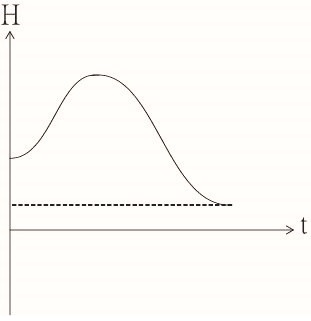
\includegraphics[width=\linewidth, center]{放熱.jpg}
\caption{放熱反應, 其$\rm \Updelta H<0 \rightarrow$放熱}
\label{fig:exothermal}
\end{minipage}%
\begin{minipage}{0.5\textwidth}
\centering
\graphicspath{{chemistry/}}
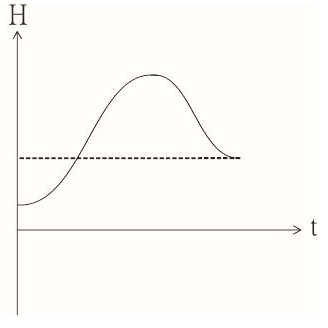
\includegraphics[width=\linewidth, center]{吸熱.jpg}
\caption{吸熱反應, 其$\rm \Updelta H>0 \rightarrow$吸熱}
\label{fig:endthermal}
\end{minipage}
\end{figure}

\section{熱反應式及標準狀態}
\subsection{熱反應式表示式}
	\begin{enumerate}
	\item $\rm \mbox{反應物}+\Updelta H \rightarrow \mbox{生成物}$
	\item $\rm \mbox{反應物}\rightarrow \mbox{生成物} \, \, \Updelta \rm H = x \rm \, kcal$(此種表示較常使用)
	\end{enumerate}
\subsection{標準狀態(standard state)}
標準狀態為在一大氣壓力下,某一特定溫度的狀態。國際標準指在1atm 和298K (25°C)的狀態。
\section{生成熱($\rm\Updelta H^{\circ}_f$)}
\begin{enumerate}
\item 元素在標準狀態下以最穩定結構存在時,定其生成熱為0 \\
EX: 石墨(C)、白磷(P)、斜方硫(S)
\item 化合物之反應熱訂為由元素的最穩定態合成化合物的焓變化量(目標化合物之係數必為一) \\
EX: $\rm Pb_{(s)}+\frac{1}{8}S_8+2O_2 \rightarrow PbSO_{4(s)}\quad \Updelta H^{\circ}_f=-219.87 \, kcal$

\end{enumerate}
\section{燃燒熱($\rm\Updelta H^{\circ}_c$)}
$\rm \Updelta H^{\circ}_c$ 為1mol反應物和$\rm O_2$於25℃ 完全反應的焓變化量(若生成物生成時處於高溫狀態,則待其溫度降至25℃時再總計焓變化量) \\
所有放熱反應的$\rm \Updelta H^{\circ}_c$皆為負數:\\
$$\rm Hg_{(l)} + \frac{1}{2} O_2 \rightarrow HgO_{(s)} \quad \Updelta H^{\circ}_c=-21.71 \quad kcal$$

\section{赫斯定律(Hess's Law)}
\begin{enumerate}
\item 正反應與逆反應之$\Updelta \rm H$互為相反數
\item 因為能量守恆的緣故,各化學反應式的焓變化量可以加成
\item \textbf{赫斯定律(Hess's Law):} \\
若一反應為:
\begin{equation}
\rm X + \rm Y \rightarrow \rm Z \label{X+Y}
\end{equation}
且已知有兩反應為:
\begin{equation}
\rm A + B \rightarrow  X \quad \Updelta  H=\Updelta  H_1 \label{A+B}
\end{equation}
\begin{equation}
\rm C + D \rightarrow  Y \quad \Updelta  H=\Updelta  H_2 \label{C+D}
\end{equation}
將\eqref{A+B}與\eqref{C+D}相加可以得到:
\begin{equation}
\rm A+B+C+D \rightarrow  X+Y \quad \Updelta  H = \Updelta H_1 + \Updelta  H_2
\end{equation}
又因為\eqref{X+Y},我們最後可以得到:
\begin{equation}
\rm A+B+C+D \rightarrow  Z \quad \Updelta  H = \Updelta H_1 + \Updelta  H_2 
\end{equation}

\end{enumerate}
\section{其餘特殊的熱能}
\subsection{游離能}
從 1 mol 氣態原子或離子移去最易游離電子的反應熱稱為第一游離能($\rm \Updelta H^{\circ}_1$),移去兩個則稱為第二游離能($\rm \Updelta H^{\circ}_2$)
$$ \rm Na_{(g)} \rightarrow Na^{+}_{(g)}+e^- \quad \Updelta H^{\circ}_1 = 120.04 \, kcal $$
\subsection{電子親和力}
1 mol 氣態原子與 1 mol 電子結合的反應熱
$$ \rm Cl_{(g)} + e^- \rightarrow Cl^-_{(g)} \quad \Updelta \rm H^{\circ}=-87.90 \, kcal$$
\subsection{格子能}氣態離子結合並結晶成離子固體的能量
$$\rm Al^{3+}_{(g)}+3Cl^-_{(g)}\rightarrow AlCl_3 \quad \Updelta H=-1302.6 \, kcal $$
\subsection{水合能}1 mol 氣態離子與水結合成水合物的能量
$$\rm Al^{3+}_{(g)}\xlongrightarrow{H_2O} Al^{3+}_{(aq)} \quad \Updelta H=1438.0 \, kcal$$

\section{一反應式的能量圖}
\begin{figure}[H]
\graphicspath{{chemistry/}}
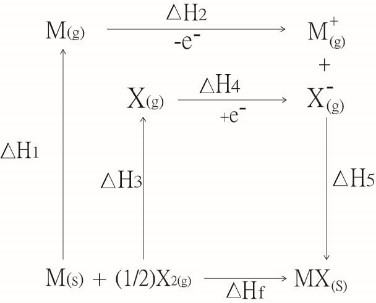
\includegraphics[width=6cm, center]{energy.jpg}
\caption{一反應式的能量圖} \vskip 10 pt
\label{fig:energy}
\end{figure}
\noindent
其中:\\
$\rm \Updelta H_1:\mbox{昇華能}$ \\ 
$\rm \Updelta H_2:\mbox{游離能}$ \\
$\rm \Updelta H_3:\frac{1}{2} \mbox{鍵解離能}$ \\ 
$\rm \Updelta H_4:\mbox{電子親和力}$ \\ 
$\rm \Updelta H_5:\mbox{格子能}$ \\ 
$\rm \Updelta H_f:\Updelta H_1+\Updelta H_2+\Updelta H_3+\Updelta H_4+\Updelta H_5$


\section{以一反應式的完整步驟計算標準反應熱 (例子)}
試求:$\rm Na_{(s)}+\frac{1}{2}Cl_{2(g)}\rightarrow NaCl_{(s)}$的標準反應熱? \\
解法:
\begin{align}
\rm Na_{(g)} \rightarrow Na^+_{(g)}+e^- \quad \Updelta H^{\circ}&=120.04 \, \rm kcal \mbox{(游離能)} \label{IE} \\
\rm Cl_{(g)}+e^- \rightarrow Cl^-_{(g)} \quad \Updelta H^{\circ}&=-87.9 \, \rm kcal \mbox{(電子親和力)} \label{E_ea} \\
\rm Na^+_{(g)}+Cl_{(g)}\rightarrow NaCl_{(s)} \quad \Updelta H^{\circ}&=-185.4 \, \rm kcal \mbox{(格子能)} \label{LE}
\end{align}
由(\ref{IE}) (\ref{E_ea}) (\ref{LE}) 相加可得:
\begin{align}
\rm Na_{(g)} + Cl_{(g)} \rightarrow NaCl_{(s)} \quad \Updelta H^{\circ}&=-153.3 \, \rm kcal \label{com}
\end{align}
接著:
\begin{align}
\rm Na_{(s)} \rightarrow Na_{(g)} \quad \Updelta H^{\circ}&=25.98 \, \rm kcal \mbox{(昇華能)} \label{SHE} \\
\rm \frac{1}{2} Cl_{2(g)} \rightarrow Cl_{(g)} \quad \Updelta H^{\circ}&=29.082 \, \rm kcal (\frac{1}{2} \mbox{鍵解離能}) \label{BE}
\end{align}
將(\ref{com})(\ref{SHE})(\ref{BE})相加可得
\begin{align}
\rm Na_{(s)}+\frac{1}{2}Cl_{2(g)}\rightarrow NaCl_{(s)} \quad \Updelta H^{\circ}&=-98.2 \, \rm kcal
\end{align}
\section{附錄}
\subsection{符號一覽表:}
	\begin{itemize}
	\item $\Delta$:變化量(末減初)
	\item $\rm \Updelta H$:焓變化量
	\item $\rm\Updelta H^{\circ}_f$:生成熱
	\item $\rm\Updelta H^{\circ}_c$:燃燒熱
	\item $\rm \Updelta H^{\circ}$:標準狀態時的焓變化量
	\item (s):固態, (l):液態, (g):氣態, (aq):水溶液, 水合物
	\item $\rm e^-$:電子
	\item $\rm Pb$:鉛, $\rm S$:硫, $\rm O$:氧, $\rm PbSO_4$:硫酸鉛, $\rm Hg$:汞, $\rm HgO$:氧化汞, $\rm Al$:鋁
	\end{itemize}
\subsection{$\rm W=-P \Updelta V$ 的推導:} \label{w=pv}
\noindent
\textbf{由功的定義:} \\
$$\rm W = F \cdot x $$ 
\textbf{我們可以令:} 
\begin{gather*}
\rm W=F \cdot \Updelta x=PA \Updelta x \\
\rm \Updelta V = -A \cdot \Updelta x
\end{gather*}
\textbf{因此有:} \\ 
\begin{gather*}
\boxed{\rm W =-P\Updelta V} \\
\mbox{(在此狀況中,體積為縮減的,固帶負號)}
\end{gather*}
\subsection{離子鍵與共價鍵的能量關係:}
	\subsubsection{離子鍵為兩原子對電子的吸引力相差的非常大時所產生的,反之,共價鍵為兩原子對電子的吸引力差距不大時所形成的。}
	\subsubsection{若一化合物為離子化合物:}
	$$ \rm \Updelta H_f < 0 $$ \\
	原因:因為此化合物生成時為放熱反應,故在能量上是有利於反應進行
	\subsubsection{若一化合物為共價化合物:}
	$$ \rm \Updelta H_f > 0 $$ \\
	原因: 因為此化合物生成時為吸熱反應,故在能量上是不利於反應進行

	
\newpage
\subsection{常用標準生成熱表:}
\begin{longtable}{|c|c|c|}
\hline
\textbf{化學物質} & \textbf{分子式} & $\rm\Updelta H^{\circ}_f(kJ/mol)$ \\ \hline
氨(aq)         & $\rm NH_3$          & -80.8                   \\ \hline
氨(g)          & $\rm NH_3$          & -46.1                   \\ \hline
碳(石墨)         & C            & 0                       \\ \hline
碳(金剛石)        & C            & 1.9                     \\ \hline
碳(g)          & C            & 718.9                   \\ \hline
一氧化碳          & CO           & -110.6                  \\ \hline
二氧化碳(g)       & $\rm CO_2$          & -393.8                  \\ \hline
二氧化碳(aq)      & $\rm CO_2$          & -413.2                  \\ \hline
碳酸鈉           & $\rm Na_2CO_3$       & -1131                   \\ \hline
氯化鈉(aq)       & NaCl         & -407                    \\ \hline
氯化鈉(s)        & NaCl         & -411.12                 \\ \hline
氯化鈉(l)        & NaCl         & -385.92                 \\ \hline
水(g)          & $\rm H_2O$          & -242                    \\ \hline
氫氧化鈉(aq)      & NaOH         & -469.6                  \\ \hline
氫氧化鈉(s)       & NaOH         & -426.7                  \\ \hline
硝酸鈉(aq)       & $\rm NaNO_3$        & -446.2                  \\ \hline
硝酸鈉(s)        & $\rm NaNO_3$        & -424.8                  \\ \hline
二氧化硫          & $\rm SO_2$          & -297                    \\ \hline
二硫化碳(l)       & $\rm CS_2$          & -89.41                  \\ \hline
二硫化碳(g)       & $\rm CS_2$          & -117.1                  \\ \hline
硫酸            & $\rm H_2SO_4$        & -814                    \\ \hline
二氧化矽          & $\rm SiO_2$         & -911                    \\ \hline
二氧化氮          & $\rm NO_2$          & 33                      \\ \hline
一氧化氮          & NO           & 90                      \\ \hline
水(l)          & $\rm H_2O$          & -286                    \\ \hline
氯化鈉(g)        & NaCl         & -181.42                 \\ \hline
氫             & $\rm H_2$           & 0                       \\ \hline
氟             & $\rm F_2$           & 0                       \\ \hline
氯             & $\rm Cl_2$          & 0                       \\ \hline
溴(l)          & $\rm Br_2$          & 0                       \\ \hline
溴(g)          & $\rm Br_2$          & 31                      \\ \hline
碘(s)          & $\rm I_2$           & 0                       \\ \hline
碘(g)          & $\rm I_2$           & 62                      \\ \hline
\end{longtable}


\section{講師介紹}
\begin{itemize}
\item 姓名:張竣程
\item 性別:男
\item 特色:上課時通常不是在睡覺就是在看漫畫(編按:但還是超電)、在國中時期吃遍各種顏色的粉筆(編按:可以詢問講師他覺得哪一種顏色的粉筆比較好吃喔),甚至是蝴蝶、聽說在科班入學考試中拿到第二名的成績、熟捻所有周星馳電影,能將台詞及角色倒背如流。
\item 名言:考試靠賽,輕鬆自在、我以後要當尼特族!!!
\end{itemize}